\documentclass[main.tex]{subfiles}

\begin{document}
	
	В данном разделе приводятся схемы работы алгоритмов:
	
\subsection{Алгоритмы}
	
	\begin{enumerate}[1)]
		\item перебором \ref{fig:1} \ref{fig:1.1};
		\item муравьиный \ref{fig:2} \ref{fig:2.1} \ref{fig:2.2}. 
	\end{enumerate}

	\begin{figure}[H]
		\centering
		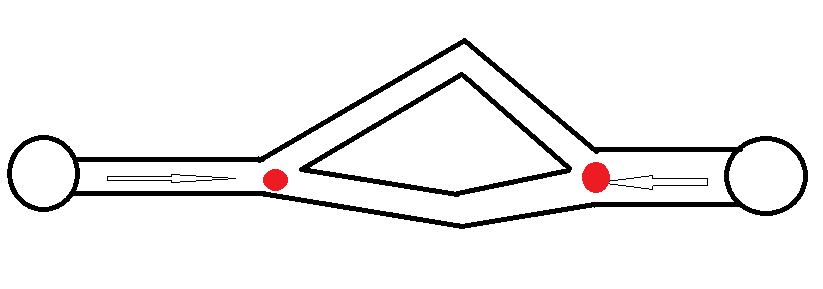
\includegraphics[scale=0.5]{src/img/1}
		\caption{Нахождение решения перебором}
		\label{fig:1}
	\end{figure}
	
	\begin{figure}[H]
		\centering
		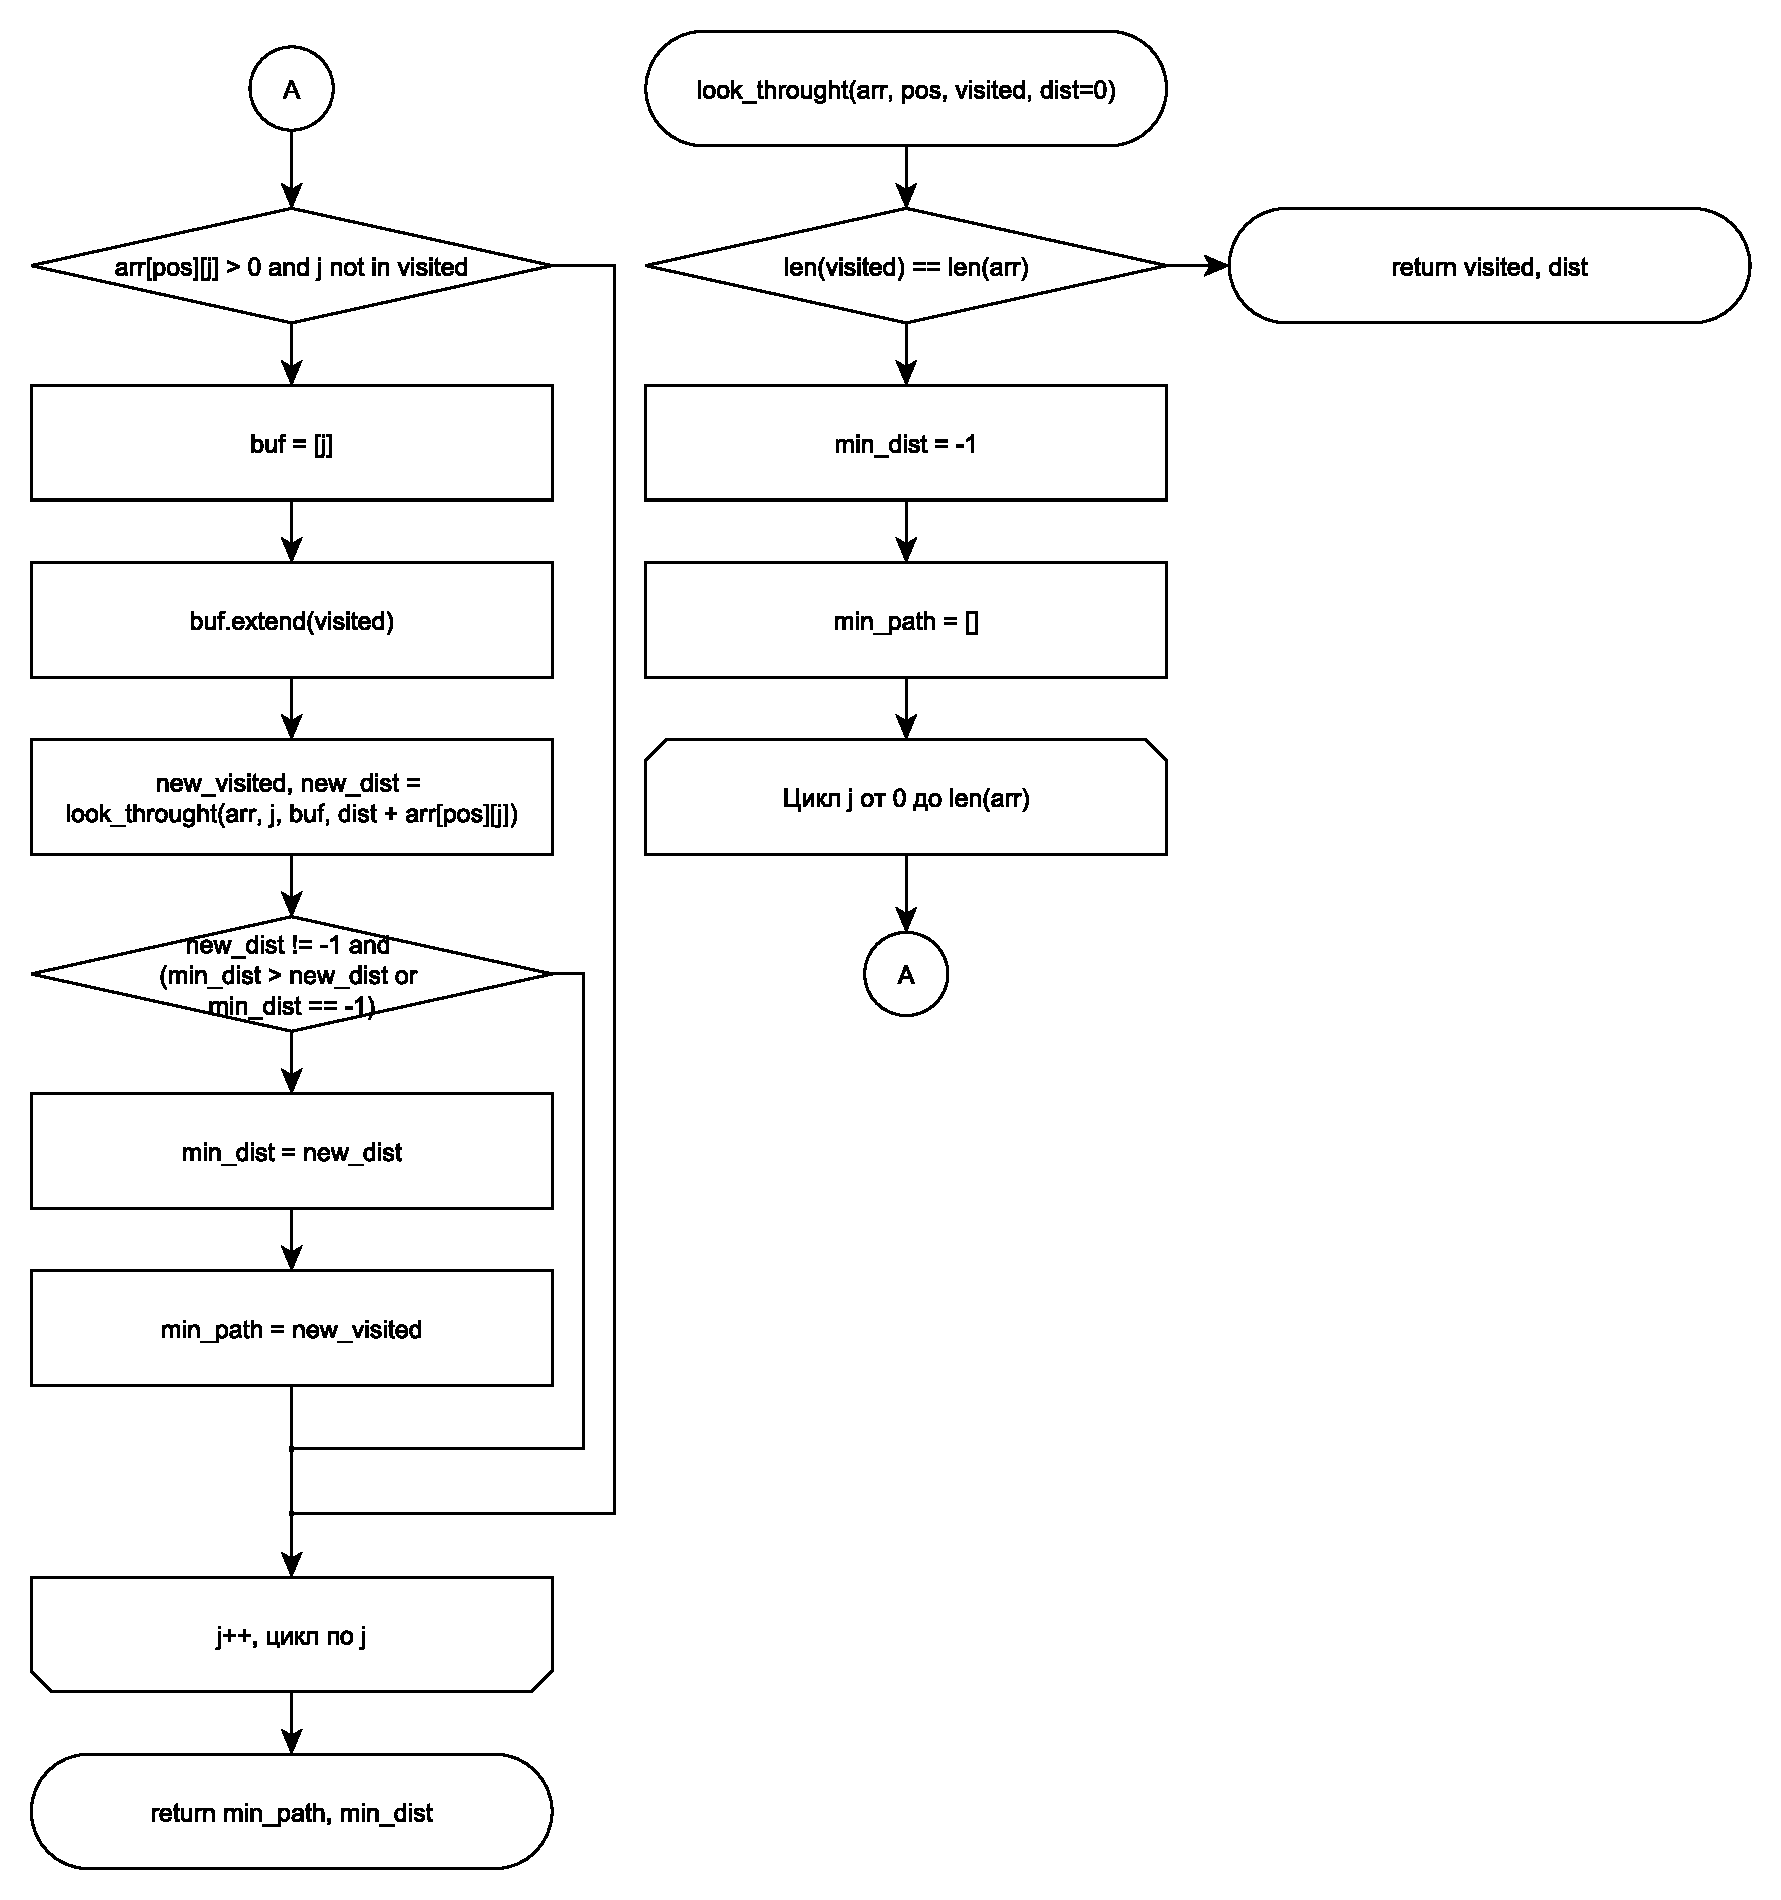
\includegraphics[scale=0.5]{src/img/1.1}
		\caption{Нахождение решения перебором}
		\label{fig:1.1}
	\end{figure}

	\begin{figure}[H]
		\centering
		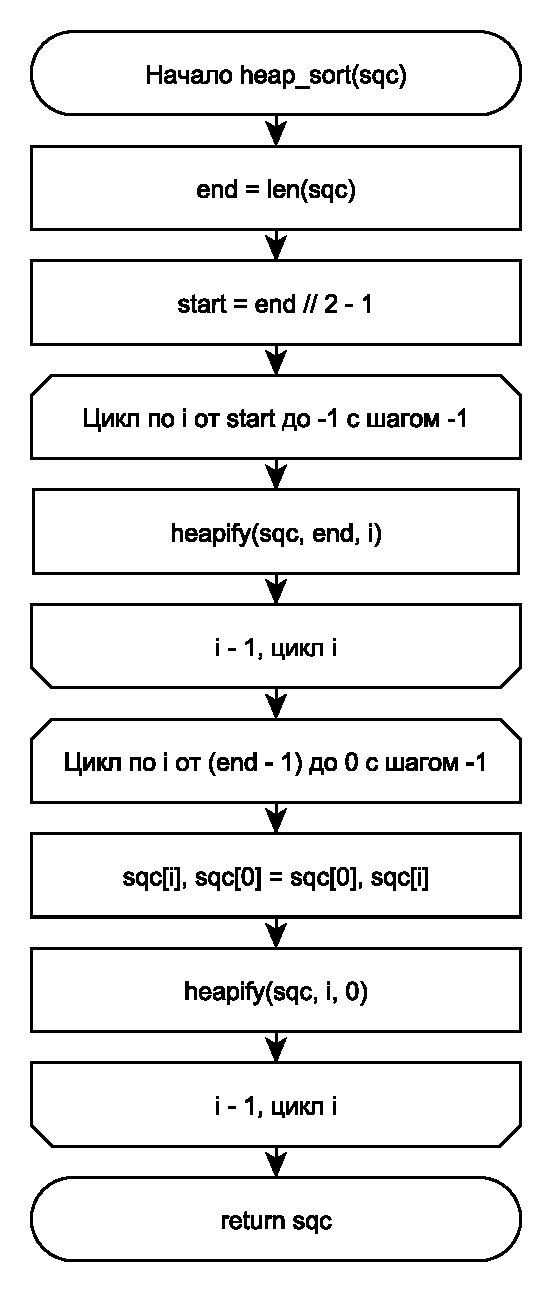
\includegraphics[scale=0.5]{src/img/2.pdf}
		\caption{Муравьиный алгоритм}
		\label{fig:2}
	\end{figure}

	\begin{figure}[H]
		\centering
		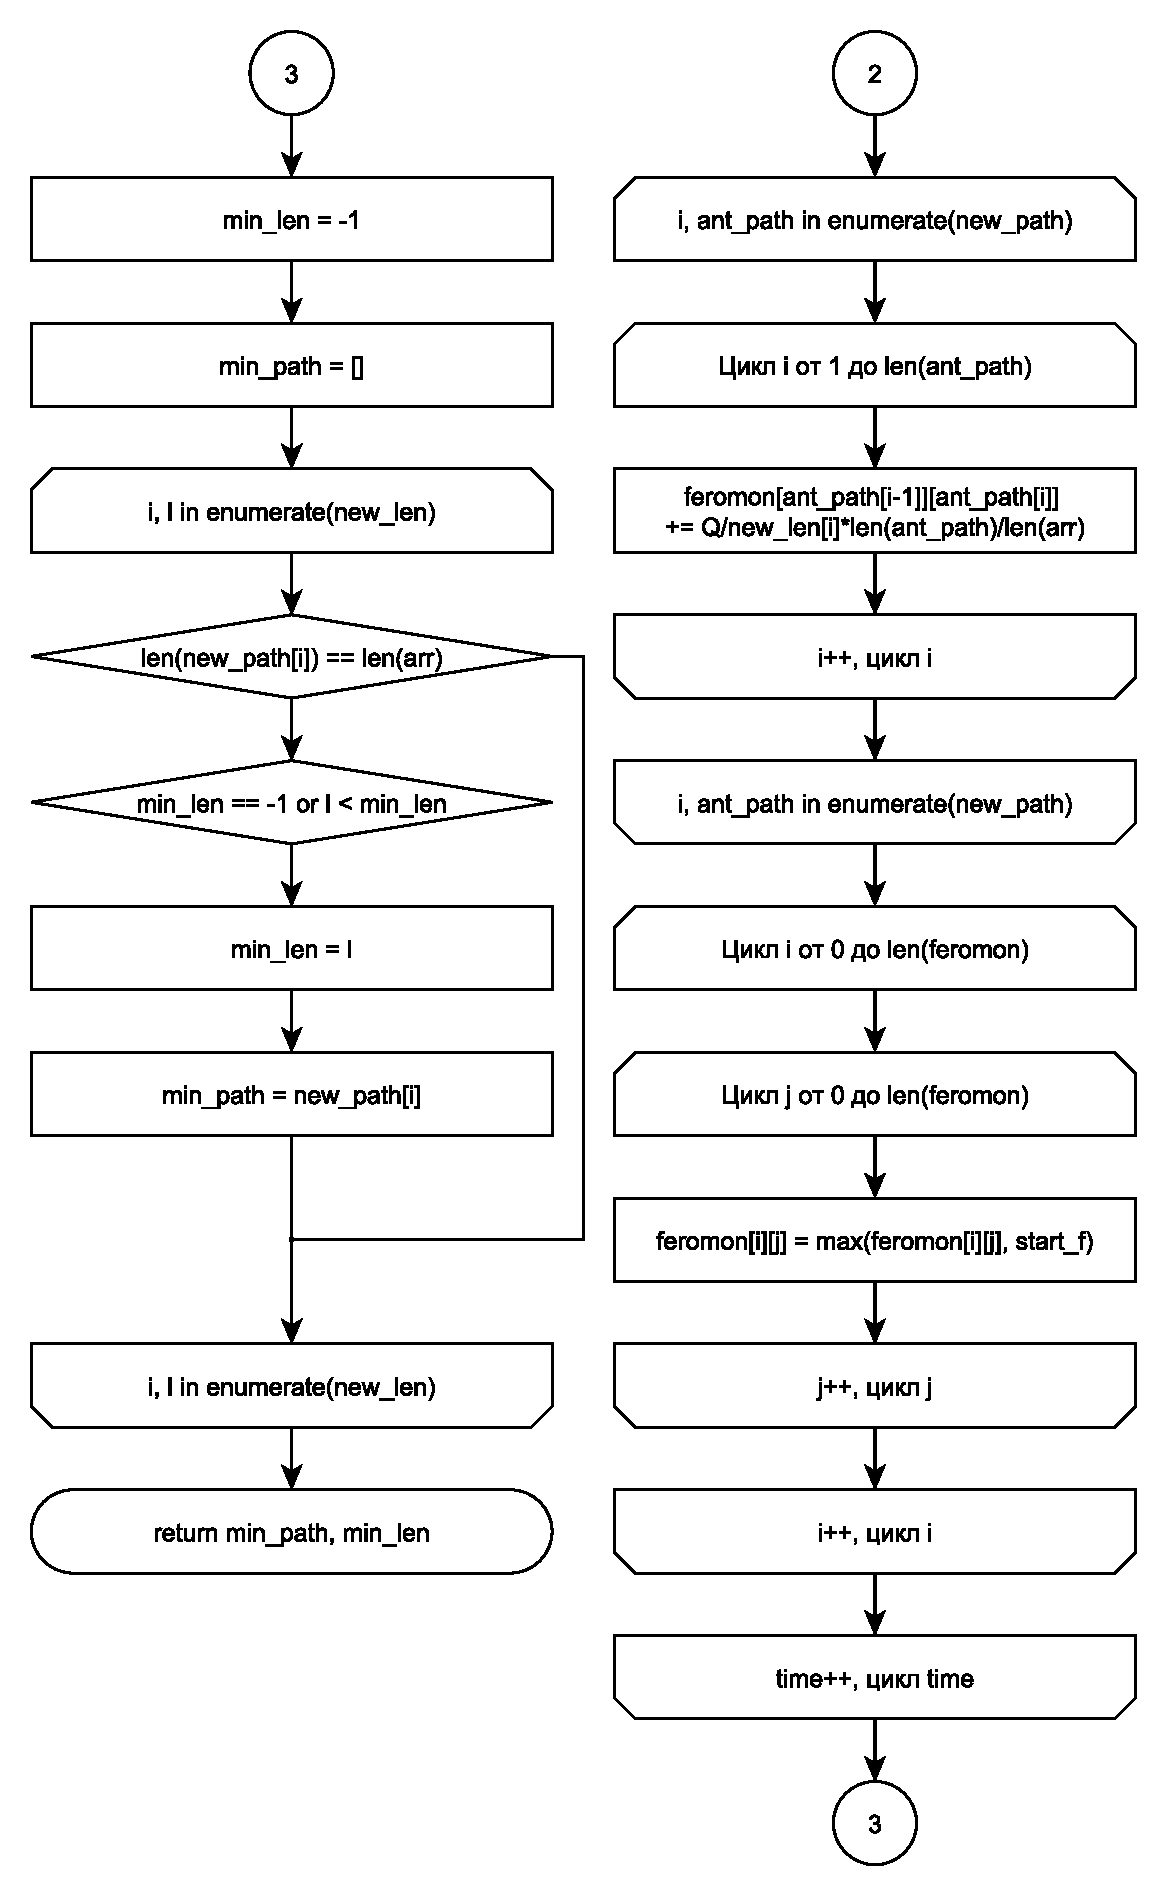
\includegraphics[scale=0.5]{src/img/2.1}
		\caption{Муравьиный алгоритм}
		\label{fig:2.1}
	\end{figure}

	\begin{figure}[H]
		\centering
		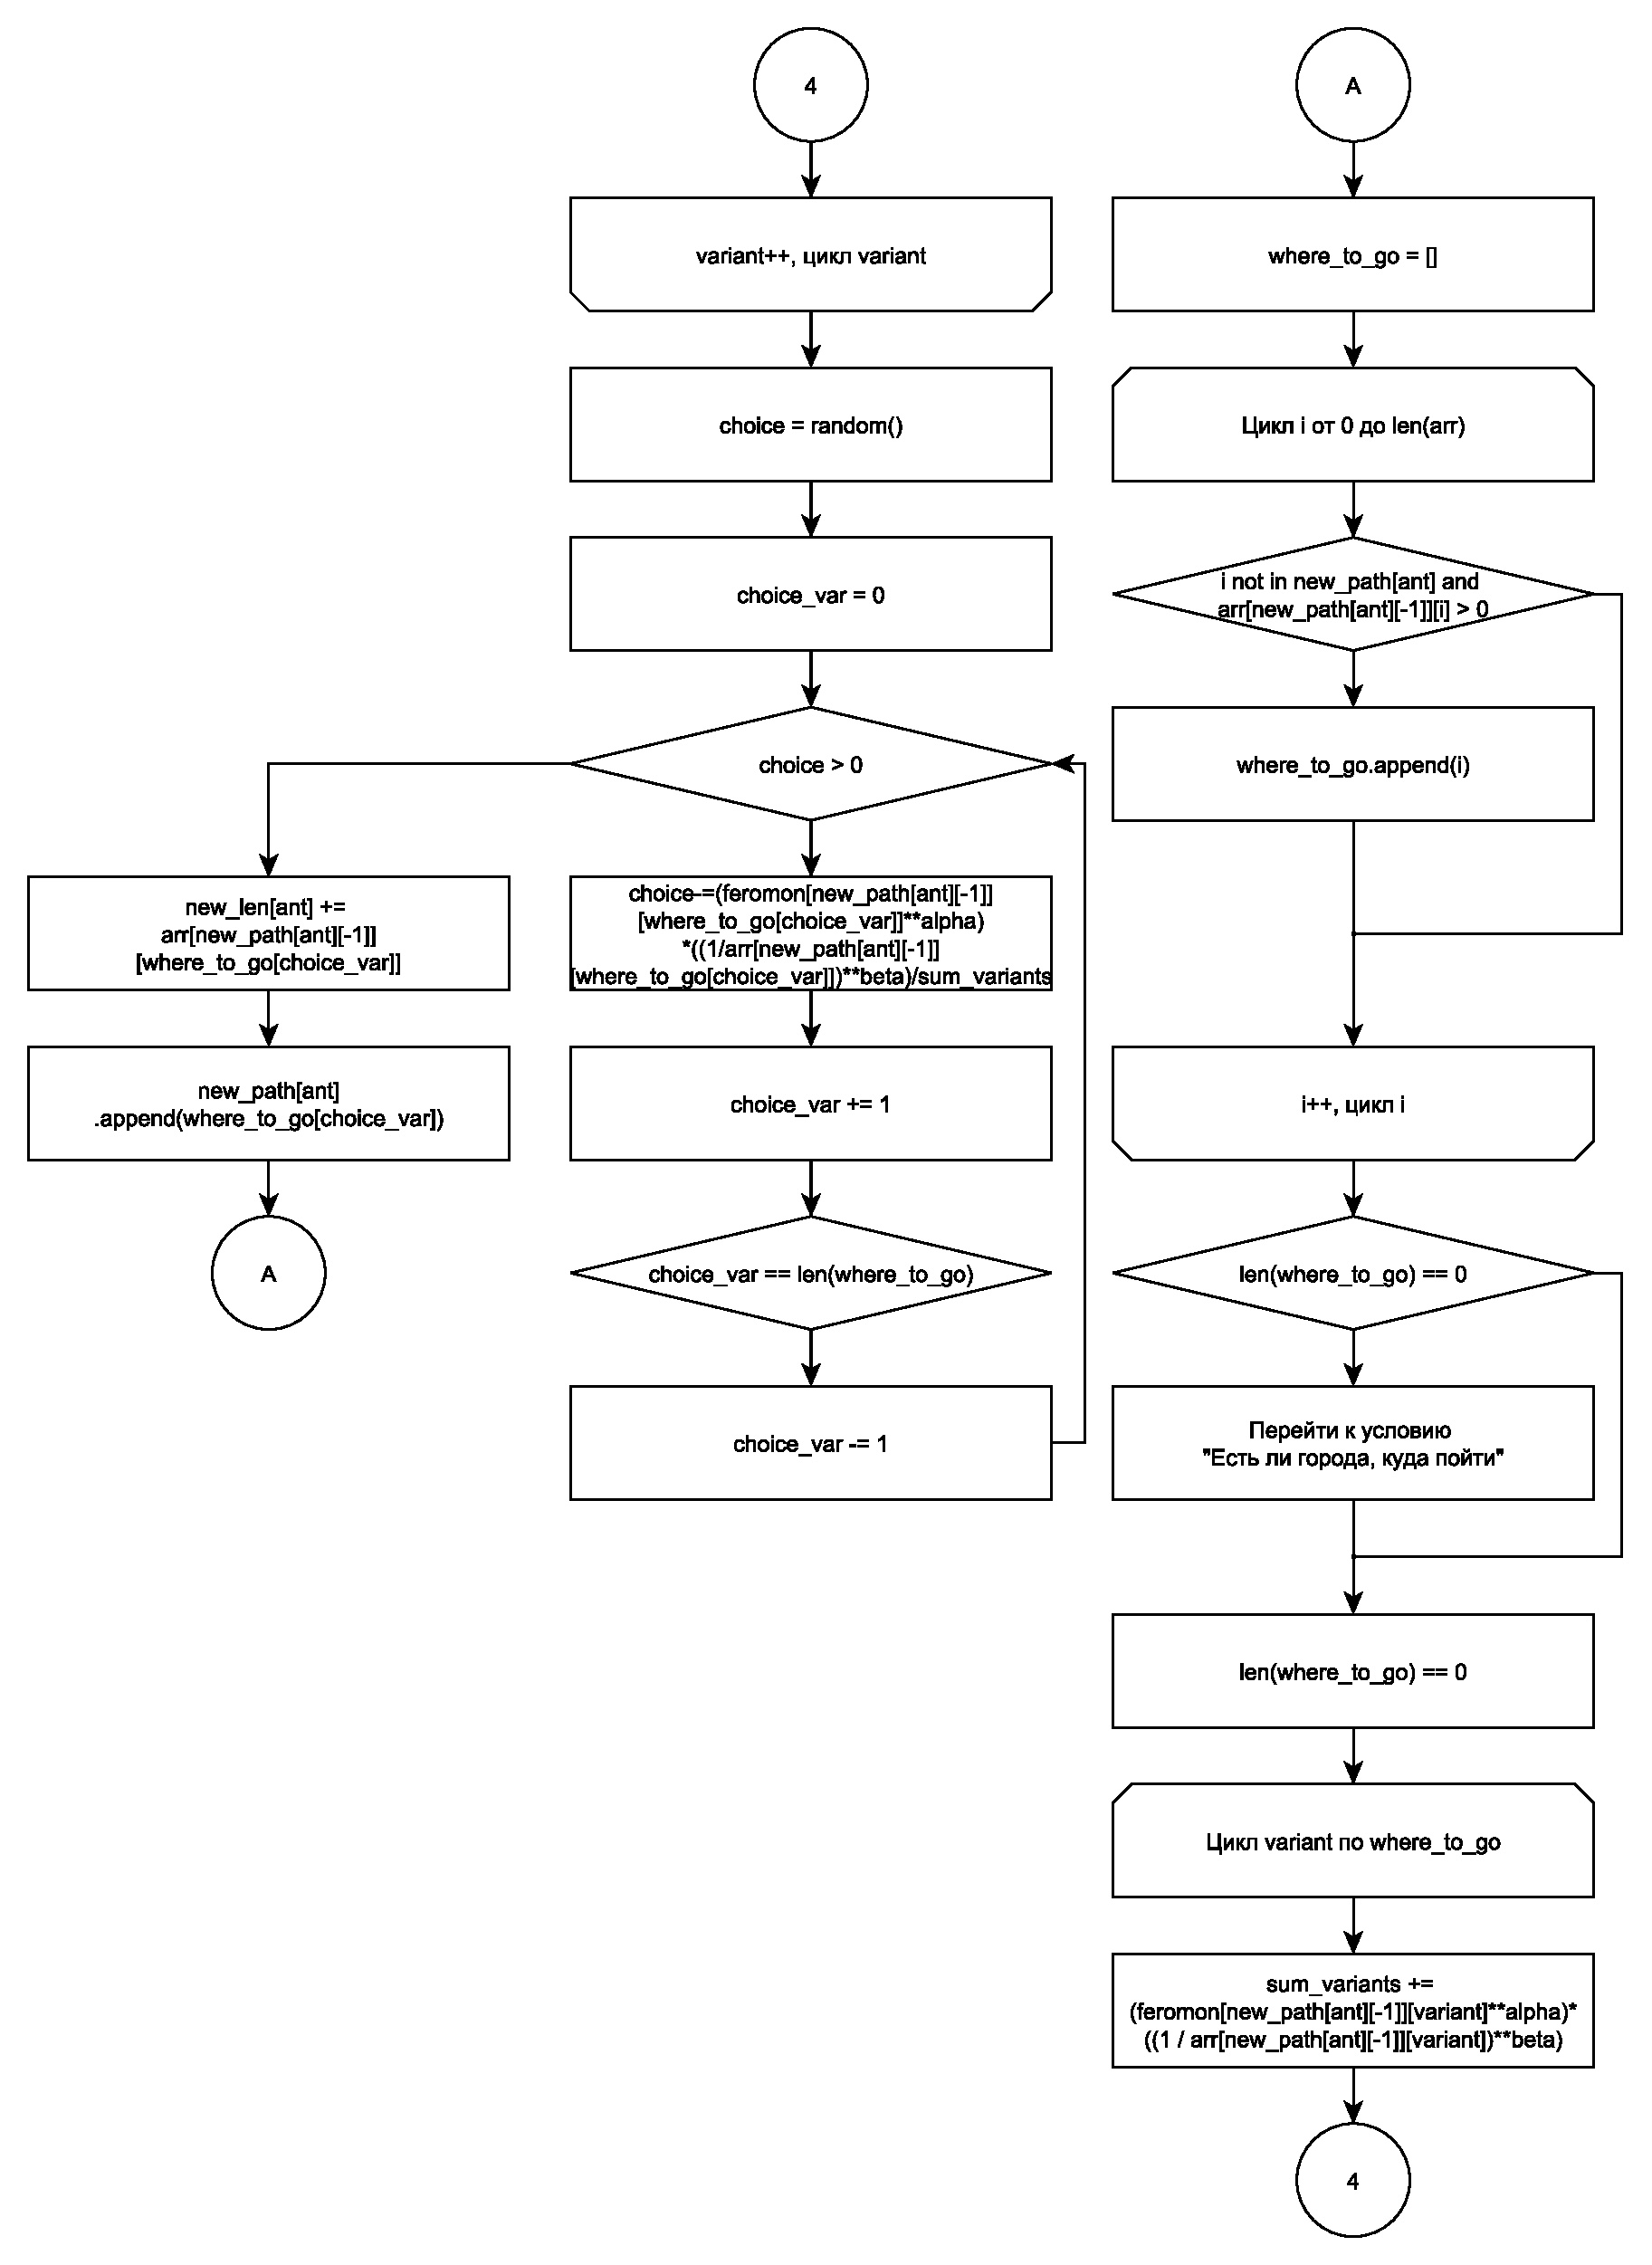
\includegraphics[scale=0.5]{src/img/2.2}
		\caption{Муравьиный алгоритм}
		\label{fig:2.2}
	\end{figure}
	
	В данном разделе приведены схемы алгоритмов
		
\end{document}